\subsubsection{Composição dos modelos genéricos}
A composição construtiva atribuída aos modelos utilizados neste trabalho mostra fundamentalmente os parâmetros necessários para a avaliação do desempenho energético segundo o INI-C. Os atributos utilizados serviram como ponto de partida para as análises subsequentes sugeridas nas etapas metodológicas e estão dispostos no Fluxograma da Figura \ref{fig:figura8}.\vspace{-0.10cm}%\pagebreak % disclaimer: não modificar pagebreak, pois é importante para manter a figura legível e as tabelas e elementos subsequentes nos seus devidos lugares.
    %\vspace*{-1cm}
    \begin{figure}[H]
        \centering
        \caption{Fatores utilizados como parâmetros de configuração volumétrica dos modelos genéricos.}
        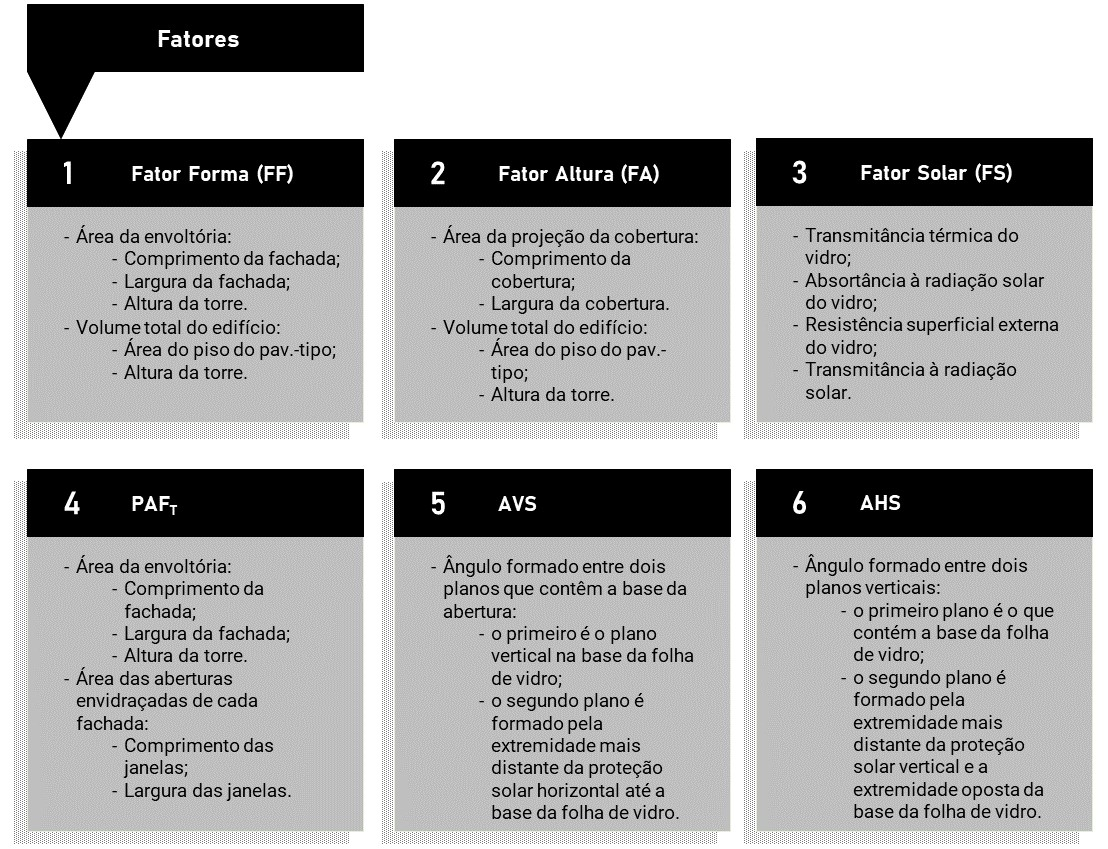
\includegraphics[width=0.9\textwidth]{figures/fig10_Fluxogramas-2.jpg}
        \begin{flushleft}
            \par \small Fonte: autor (2019)
        \end{flushleft}
        \label{fig:figura8}
    \end{figure}
\noindent Apresentados na Tabela 7 e exemplificado na Figura \ref{fig:figura9}, os atributos estudados foram Fator de Forma, FF, Fator Altura, FA, Percentual de Área de Abertura da Fachada Total, PAFT, Ângulo Vertical de Sombreamento, AVS, e Ângulo Horizontal de Sombreamento, AHS.%\vspace*{0.3cm}
\begin{figure}[H]
    \centering
    \caption{Estrutura arquitetônica dos modelos genéricos.}
    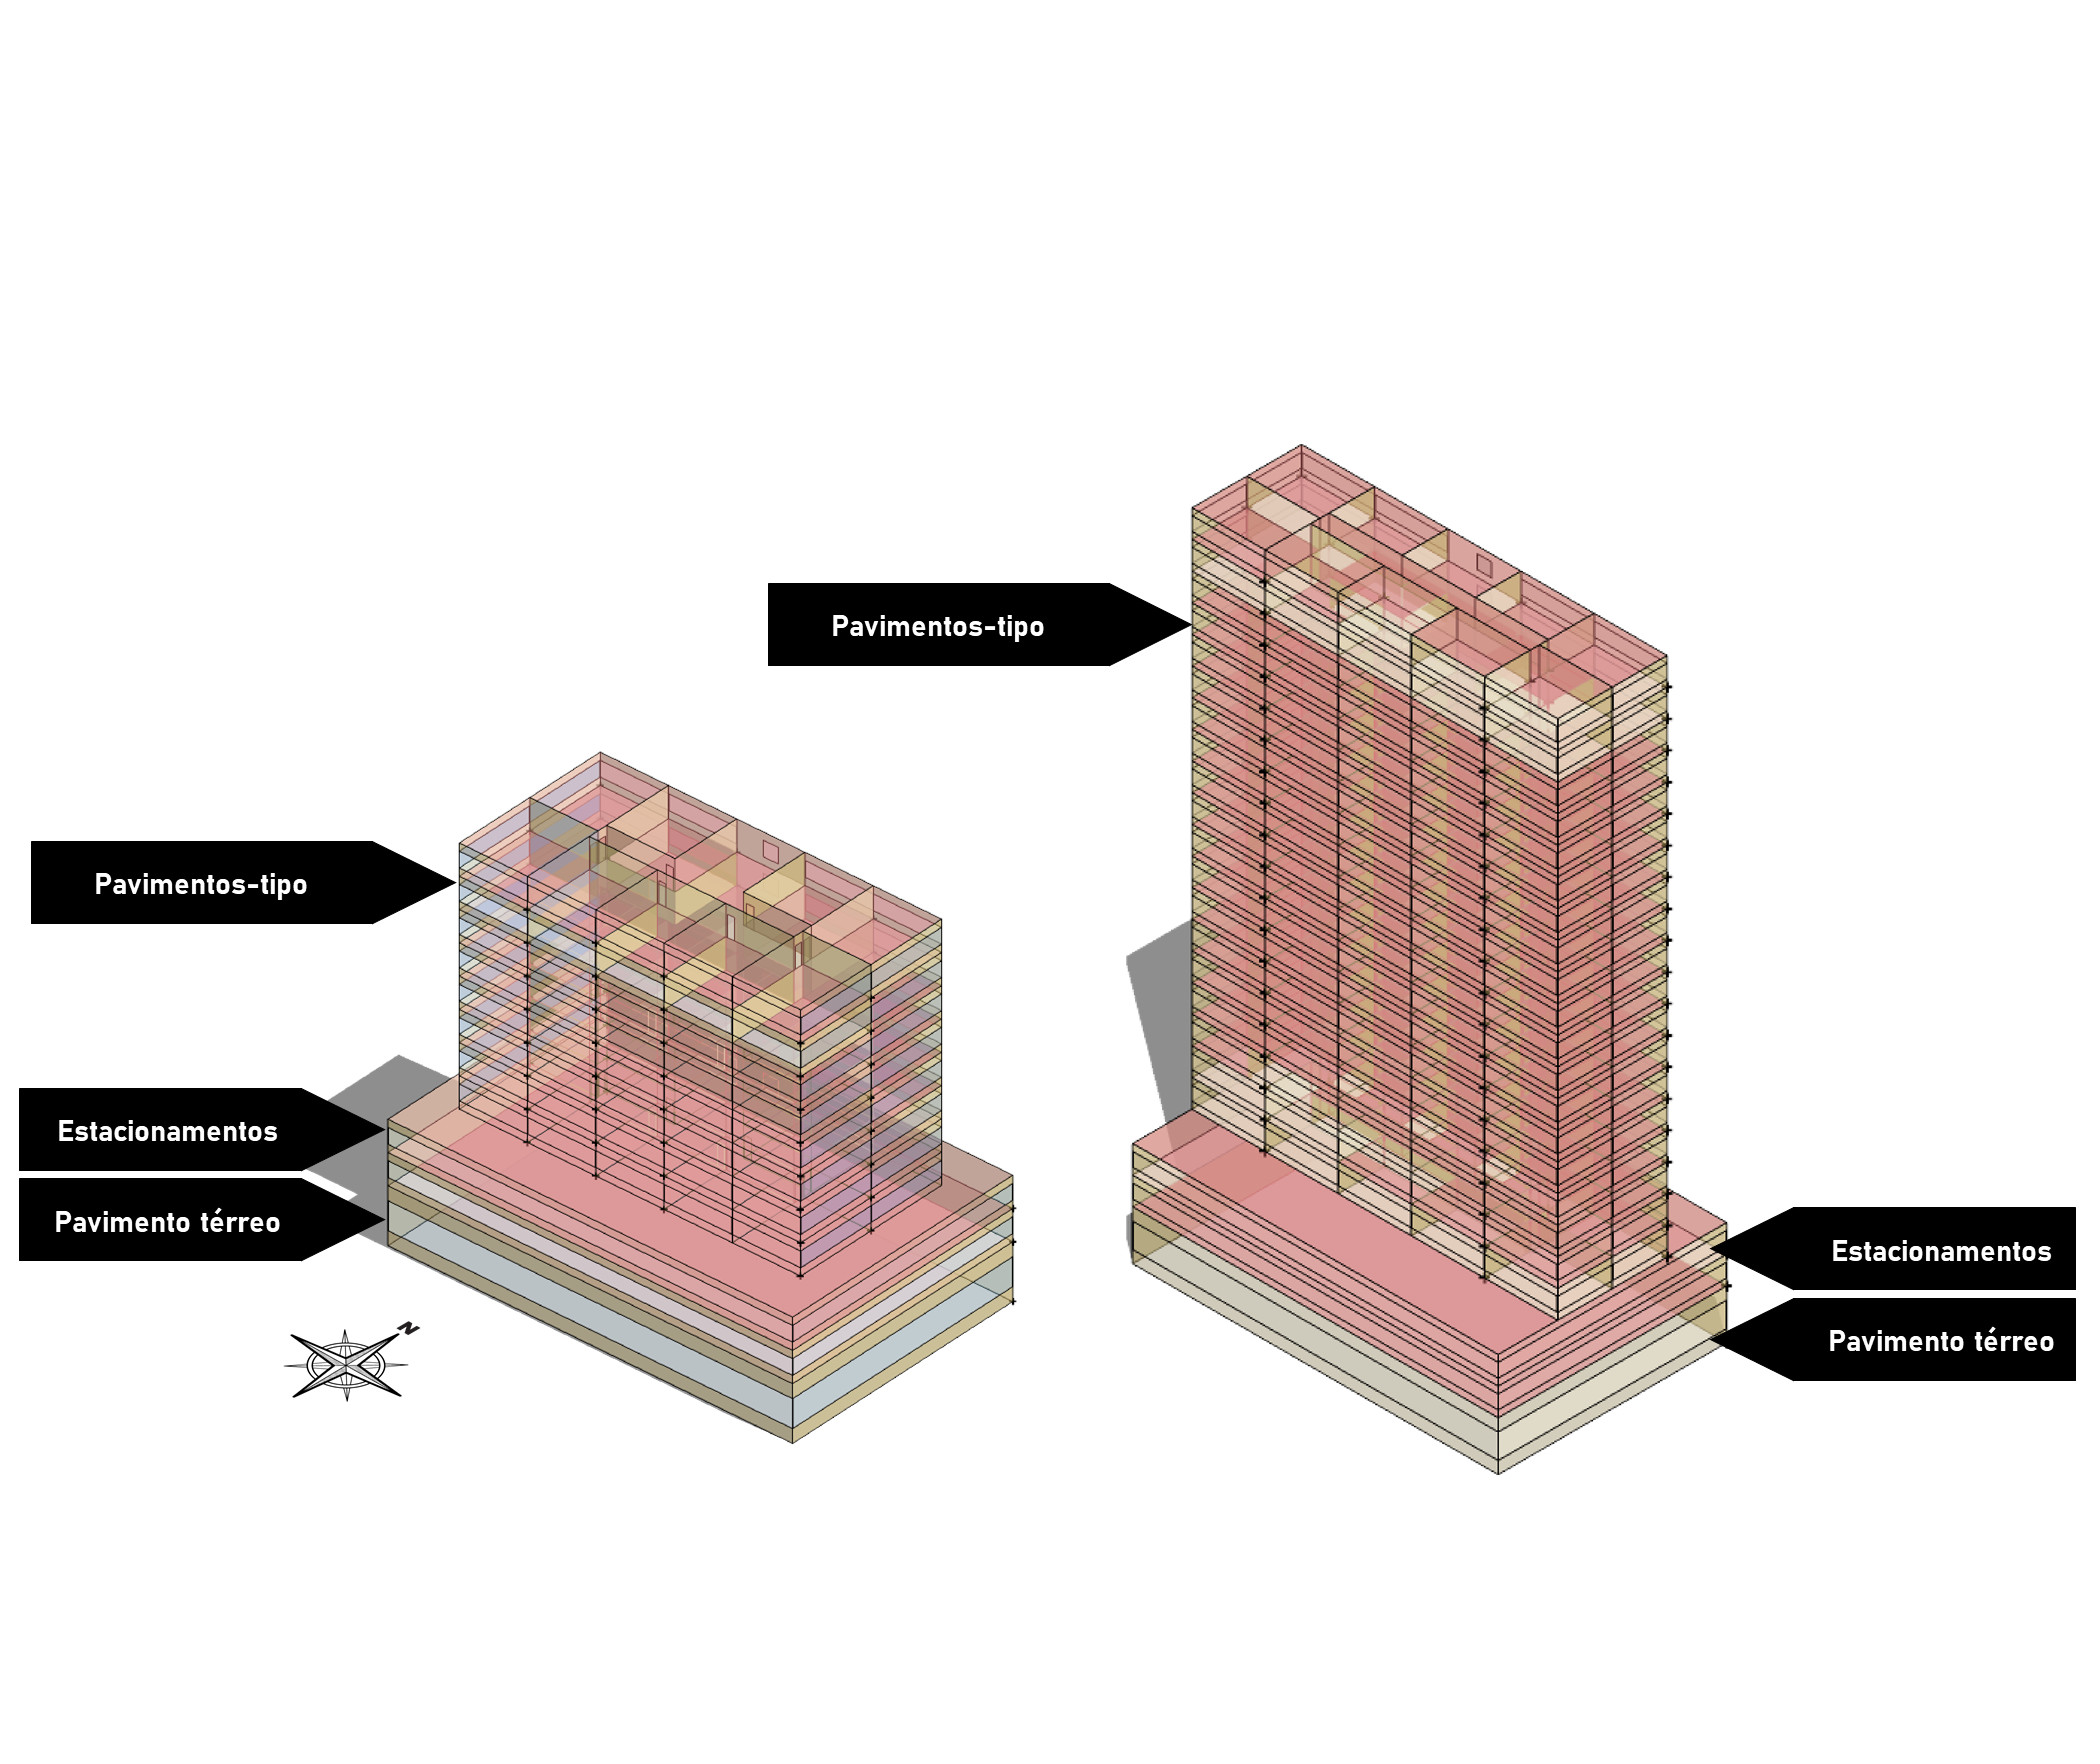
\includegraphics[width=0.9\textwidth]{figures/fig11_8-19-2pav.png}
    \begin{flushleft}
        \par \small Fonte: autor (2019).
    \end{flushleft}
    \label{fig:figura9}
\end{figure}
\noindent O PAF\textsubscript{T} e as propriedades do vidro utilizados para os modelos genéricos, como Fator Solar – FS, ou Solar Heat Gain Coefficient – SHGC, foram adotados considerando as médias desses atributos coletados in loco e complementados por dados extraídos do Catálogo de Propriedades Térmicas e Óticas de Vidro \cite{CentroBrasileirodeEficienciaEnergeticaemEdificacoesCB3E2015,AssociacaoBrasileiradeNormasTecnicas-ABNT2003}, da NBR 15220 (2003) e do INI-C \cite{InstitutoNacionaldeMetrologiaNormalizacaoeQualidadeIndustrial-INMETRO2018}, como forma de tornar genéricos os dados empregados, como apresentado na Tabela \ref{tab:tabela8}.%\vspace*{0.3cm} \newline
\begin{table}[H]
    \centering
    \small
    \caption{Parâmetros arquitetônicos dos modelos genéricos.}
    \begin{tabular*}{\columnwidth}{@{\extracolsep{\fill}}l|ll}
    \hline
    \textbf{Parâmetro}                                                              & \textbf{Descrição}         & \textbf{Referências}  \\ \hline
    \multicolumn{3}{c}{\textbf{Dados dimensionais dos pavimentos-tipo}}\\\hline
    Número de pavimento (un)                                                        & 8                          & 19                    \\ \hline
    \makecell[l]{Proporção geométrica – pav.\\ tipo (m – Comprimento x Largura)}    & 33,75x16                   & 40x12                 \\ \hline
    Altura do pavimento-tipo (m)                                                    & 3                          & 3                     \\ \hline
    \makecell[l]{Área total construída – pavimentos-tipo (m²)}                      & 4.320                      & 9.120                 \\ \hline
    Área de projeção da cobertura - Apcob (m²)                                      & 843,75                     & 640,00                \\ \hline
    Área de projeção do edifício - Ape (m²)*                                        & 1000                       & 1000                  \\ \hline
    Área total construída - Atot (m²)                                               & 7.320                      & 12.120                \\ \hline
    Volume Total da Edificação - Vtot (m³)                                          & 24.360                     & 38.760                \\ \hline
    Área da envoltória - Aenv (m²)                                                  & 5.430,30                   & 8.890,00              \\ \hline
    Fator de Forma (FF)                                                             & 0,222                      & 0,229                 \\ \hline
    Fator Altura (FA)                                                               & 0,125                      & 0,052                 \\ \hline
    Fator Solar (FS)                                                                & 0,44                       & 0,44                  \\ \hline
    Transmitância do vidro (W/m²K)                                                  & 5,6                        & 5,6                   \\ \hline
    Área de aberturas das fachadas – Aabert (m²)                                    & 1.501,80                   & 3.152,40              \\ \hline
    PAF\textsubscript{T} (\%)                                                       & 50\%                       & 50\%                  \\ \hline
    \makecell[l]{Ângulo Vertical (AVS) e Horizontal\\ (AHS) de Sombreamento (°)}    & 0                          & 0                     \\ \hline
    \end{tabular*}
    \begin{flushleft}
        \par \small Fonte: autor (2019); *A Ape contempla a área de projeção do pavimento térreo e estacionamentos.\vspace{-0.35cm}
    \end{flushleft}
    \label{tab:tabela8}
\end{table}
\noindent Segundo o INI-C, publicado pelo \textcite{InstitutoNacionaldeMetrologiaNormalizacaoeQualidadeIndustrial-INMETRO2018}, a utilização do Ângulo de Obstrução Vertical – AOV, para a simulação de obstruções solares parciais e totais são critérios opcionais que dependem da condição real levantada. Apesar da obstrução solar lateral ter sido uma condição observada em algumas edificações de Vitória, com base na observação da frequência de ocorrência, este atributo não foi considerado para o presente trabalho dada a configuração e disposição das edificações do recorte territorial em relação ao lote, que possibilitaram utilizar cenários sem obstrução solar. Além disso, para o estudo da incidência de radiação solar sobre a edificação e como ponto de partida para a implementação das estratégias passivas aos modelos genéricos, foi definido a fachada principal com orientação Sul, de acordo com a frequência de ocorrência observada na amostragem.\vspace*{0.3cm} \newline
\noindent O pavimento térreo e dois pavimentos de estacionamentos (Figura \ref{fig:figura10}), foram centralizados na base das torres em ambos os modelos, com dimensões idênticas e de forma genérica, com o intuito de evidenciar a influência sobre o consumo energético total por meio do número de pavimentos. Contudo, o uso e ocupação destas áreas se torna de baixa relevância, uma vez que as atividades de maior permanência se dão nos ambientes da torre.\vspace*{0.3cm} \newline
\noindent Estes pavimentos compreendem características arquitetônicas apresentadas em todas as edificações selecionadas em levantamento. Posteriormente, na etapa de produção de energia, foi proposto o deslocamento dos pavimentos abaixo da torre para aproveitamento de área para inserção de painéis fotovoltaicos.
\begin{figure}[H]
    \centering
    \caption{Conformação do pavimento térreo e estacionamentos.}
    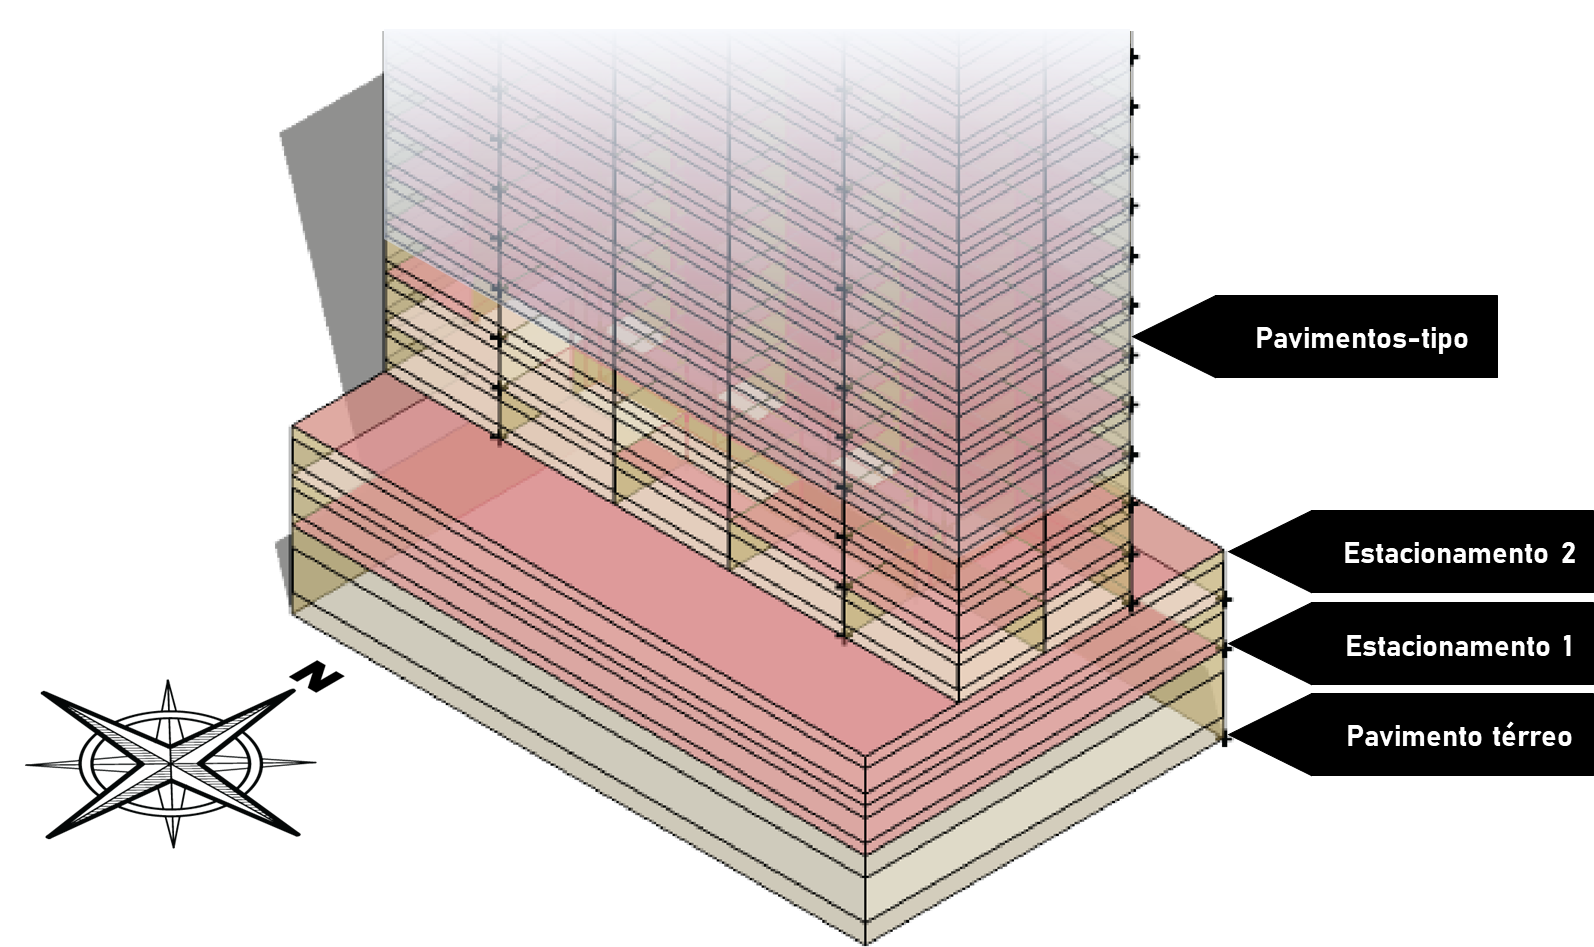
\includegraphics[width=0.9\textwidth]{figures/fig12-base_torre-1.png}
    \begin{flushleft}
        \par \small Fonte: autor (2019).
    \end{flushleft}
    \label{fig:figura10}
\end{figure}\vspace*{-0.5cm}
\noindent Os modelos são distinguidos principalmente pela área de projeção, número de pavimentos, pelo volume total e área da envoltória. Esses fatores resultam diretamente em Fator de Forma e Fator Altura distintos para cada modelo, amparando um dos objetivos específicos desta pesquisa sobre identificar as características mais influentes no consumo de energia elétrica. As zonas térmicas também formam características distintas entre os modelos genéricos, variando as áreas úteis, como apresentado na Tabela \ref{tab:tabela9}.
\begin{table}[H]
    \centering
    \small
    \caption{Zonas térmicas dos modelos genéricos.}
    \begin{tabular*}{\columnwidth}{@{\extracolsep{\fill}}ll}\hline
        \makecell[c]{Zonas térmicas - modelo\\ genérico de 8 pavimentos}                    & \makecell[c]{Zonas térmicas - modelo \\genérico de 19 pavimentos}                 \\ \hline
        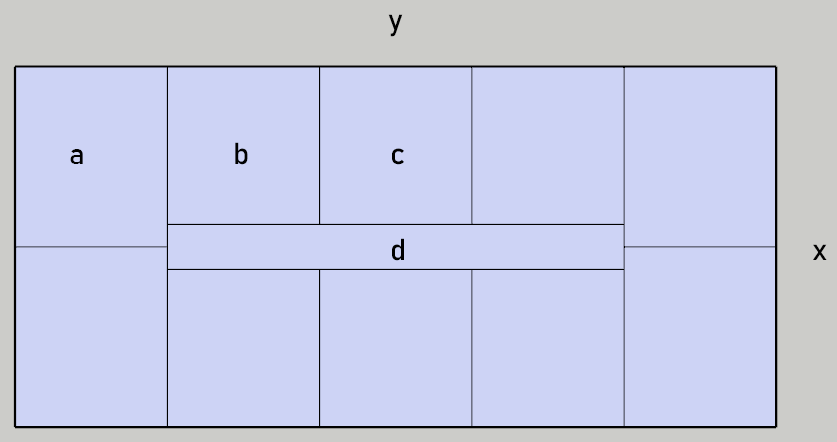
\includegraphics[width=0.5\textwidth]{figures/tab9-pb-8pav.png}                     & 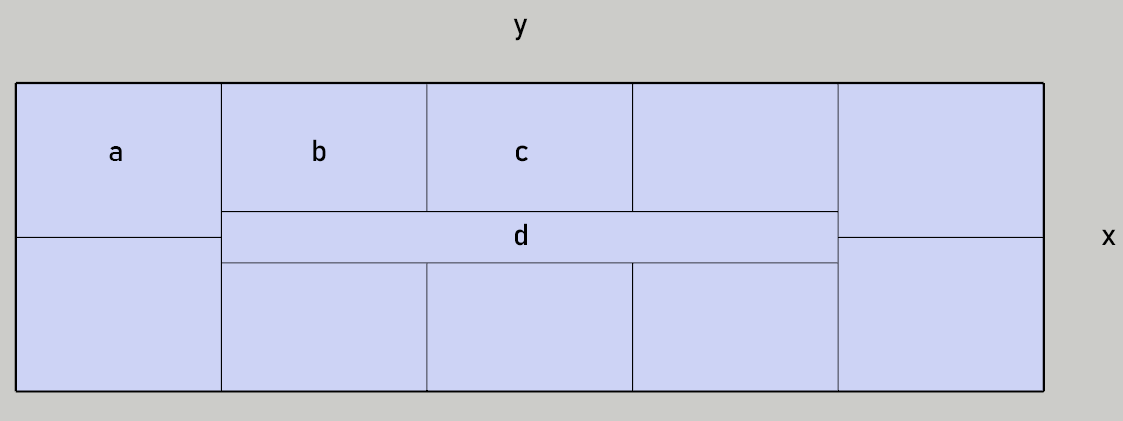
\includegraphics[width=0.5\textwidth]{figures/tab9-pb-19pav.png}                  \\
        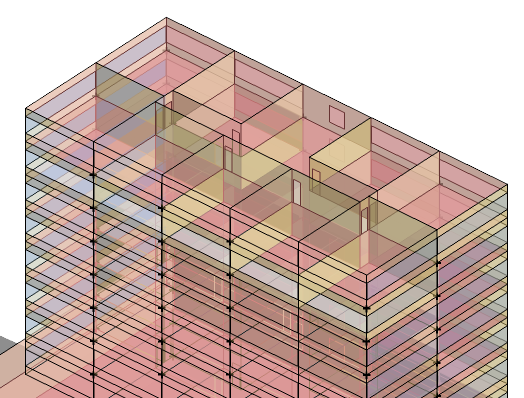
\includegraphics[width=0.5\textwidth]{figures/tab9-CEP_8pav-v3-7.png}               & 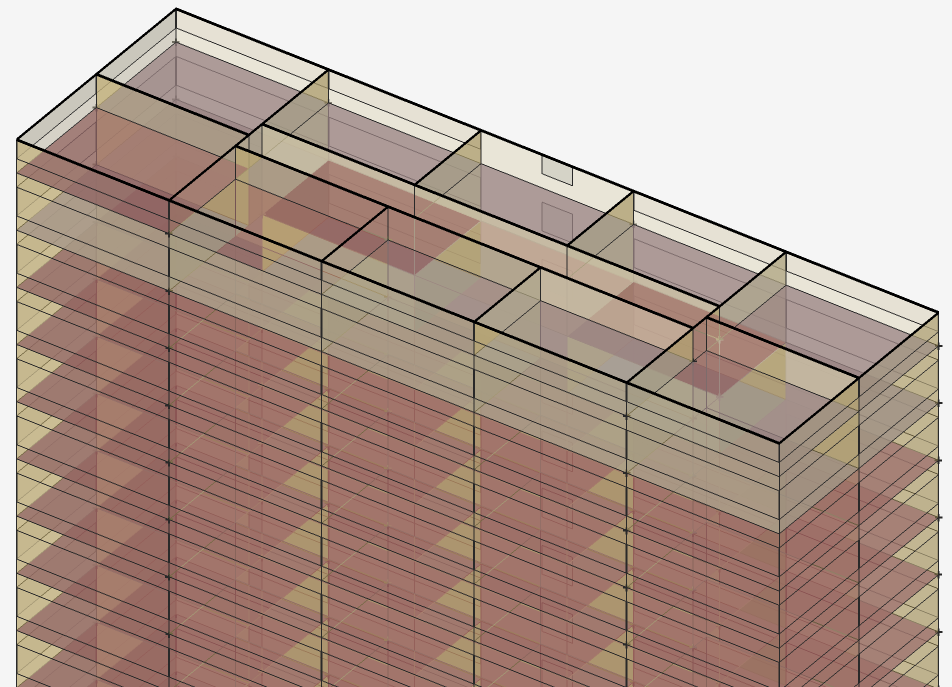
\includegraphics[width=0.5\textwidth]{figures/tab9-corte-19pav-v1.png}            \\ \hline
        Quantidade de zonas: 11                                                             & Quantidade de zonas: 11                                                           \\ \hline
        Área de projeção da torre: 843,75 m²                                                & Área de projeção da torre: 640,00 m²                                              \\ \hline
        Área da zona térmica “a”: 54,00 m²                                                  & Área da zona térmica “a”: 48,00 m²                                                \\ \hline
        Área da zona térmica “b”: 47,25 m²                                                  & Área da zona térmica “b”: 40,00 m²                                                \\ \hline
        Área da zona térmica “c+d”: 87,75 m²                                                & Área da zona térmica “c+d”: 88,00 m²                                              \\ \hline
        \makecell[l]{Largura do pavimento-tipo\\ (x): 16,00 m}                              & Largura do pavimento-tipo (x): 12,00 m                                            \\ \hline
        \makecell[l]{Comprimento do pavimento-\\tipo (y): 33,75 m}                          & \makecell[l]{Comprimento do pavimento-\\tipo (y): 40,00 m}                        \\ \hline
        \makecell[l]{Dimensões das aberturas\\ das zonas térmicas – N/S:\\ 6,70x1,51 m}     & \makecell[l]{Dimensões das aberturas das zonas\\ térmicas – N/S: 7,95x1,51 m}     \\ \hline
        \makecell[l]{Dimensões das aberturas\\ das zonas térmicas – L/O:\\ 7,95x1,51 m}     & \makecell[l]{Dimensões das aberturas das zonas\\ térmicas – L/O: 5,95x1,51 m}     \\ \hline
        \makecell[l]{Dimensões das aberturas\\ das zonas térmicas – circ.:\\ 1,49x1,51 m}   & \makecell[l]{Dimensões das aberturas das zonas\\ térmicas – circ.: 1,49x1,51 m}   \\ \hline
        \multicolumn{2}{l}{Dimensões das zonas térmicas – Pav. térreo e garagens: 40 x 25 m}                                                                                    \\ \hline
        \multicolumn{2}{l}{\makecell[l]{Dimensões das aberturas das zonas térmicas – Pav.\\ térreo e gar.: 39,95x1,51 m (N/S); 24,95x1,51 m (L/O)}}                             \\ \hline
    \end{tabular*}
    \begin{flushleft}
        \par \small Fonte: autor (2019).
    \end{flushleft}
    \label{tab:tabela9}
\end{table}
\pagebreak

\noindent Foram propostas, na etapa de otimização, proteções solares horizontais para as aberturas, que servem como proteção à radiação solar direta e controle de iluminação natural em horários predeterminados – 9, 12 e 15 horas. Este controle de horários de incidência solar se deu pelo comprimento das proteções solares propostas. Esta solução foi adotada como estratégia passiva. Utilizou-se, também, a área para proteção solar como espaço para exploração de energia solar por meio de painéis fotovoltaicos sobre os elementos protetores, como exemplificado na Figura \ref{fig:figura11} \cite{Didone2014a}.
\begin{figure}[H]
    \centering
    \caption{Painéis fotovoltaicos sobre as proteções solares da fachada oeste e cobertura.}
    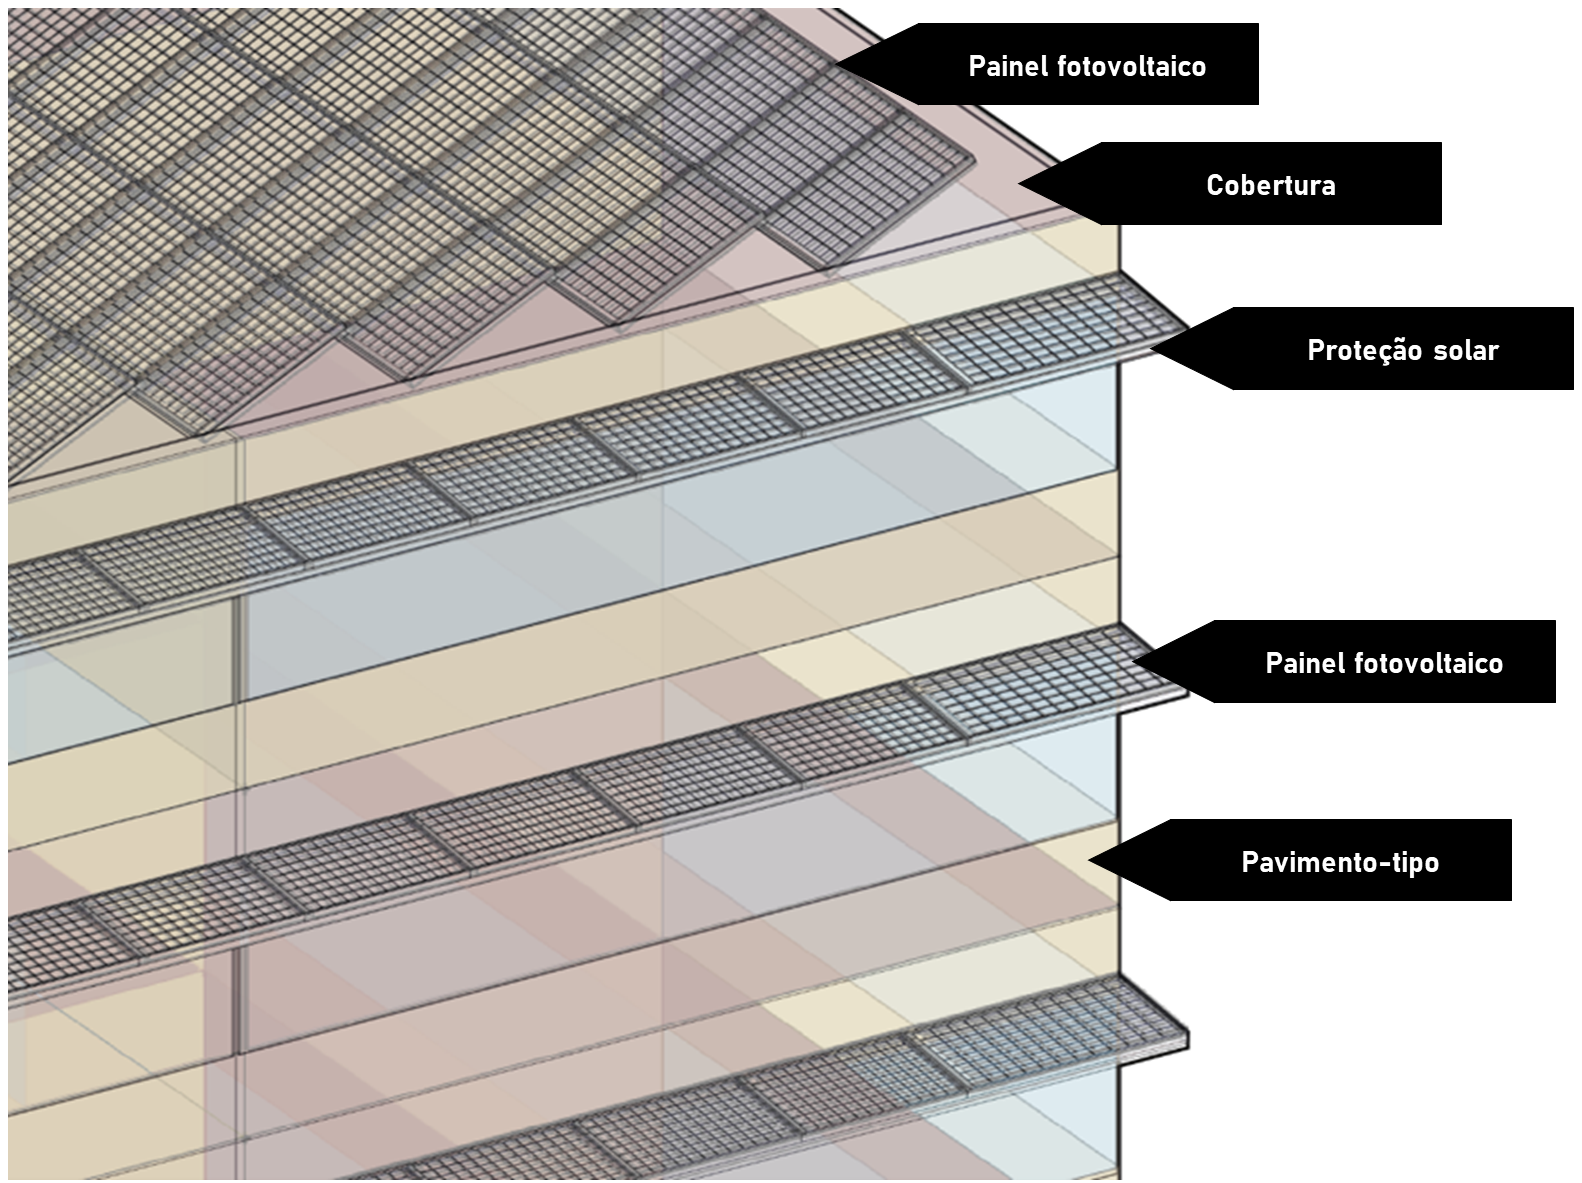
\includegraphics[width=0.9\textwidth]{figures/fig13-paineis pv.png}
    \begin{flushleft}
        \par \small Fonte: autor (2019).
    \end{flushleft}
    \label{fig:figura11}
\end{figure}